% outline:
% ---- Sahan 7 min -------
% lean basics
%    propositions
%    rewrite tactic  ~~~~ ommitted due to later examples
%      - could potentially use this to explain what a tactic is in general ~~~~~ ommitted (due to above being voided)
%    what is infoview ~ actually working with lean in vscode
% ------- Sahan -------
% Potential TODO: 
%   have
%   an analysis example (defn of limit => uniqueness of limits)

% lean examples
%    very basic examples - 2-3 maybe
%           1+x=x+1
%    odd * odd = even proof 
%    odd * odd = even proof 2
%       - talk about how differences in formalization and deciding "what is better" is an important part 

% future of our project
%    how is lean helpful, galois theory paper quote
%    potential applications/the topics we might work on
%       - quaternion algebra
%       - graph theory
%       - forms over finite fields
%       - grassmann


%  start with natural numbers
% moved to move advanced things
% even and odd function multiplied => odd function

% giving examples of math proofs converted to lean (both the real math proof, and the converted one to lean)
%    - mainly omitting the details of how the proof works in lean

% how lean works in the editor compared to other programs -- maybe mention this before talking about the examples? include a brief overview of what the "infoview" is -- we could have a slide that breaks down each part of it, i.e. how it shows variables, hypotheses, and the goal

% the future of our project, i.e. potential applications, the quote from the galois theory paper that talks about the importance of lean as a tool for working together 
\documentclass[xcolor=dvipsnames]{beamer}

\usetheme{Antibes}
\useoutertheme{miniframes} % Alternatively: miniframes, infolines, split
\useinnertheme{circles}

\definecolor{IITHorange}{RGB}{8,140,100} % orange{243, 130, 33}
\definecolor{IITHyellow}{RGB}{8,110,100} % yellow {254, 203, 10}

\definecolor{fuschia}{RGB}{12, 200, 168}
\definecolor{deep}{RGB}{52, 200, 174}
\definecolor{lace}{RGB}{52, 200, 204}
\definecolor{blush}{RGB}{42, 200, 255}

\setbeamercolor{palette primary}{bg=IITHorange,fg=white}
\setbeamercolor{palette secondary}{bg=IITHorange,fg=white}
\setbeamercolor{palette tertiary}{bg=IITHorange,fg=white}
\setbeamercolor{palette quaternary}{bg=IITHorange,fg=white}
\setbeamercolor{structure}{fg=IITHorange} % itemize, enumerate, etc
\setbeamercolor{section in toc}{fg=IITHorange} % TOC sections

% Change example block colors

% 1- Block title (background and text)
\setbeamercolor{block title example}{fg=white, bg=gray}

% 2- Block body (background)
\setbeamercolor{block body example}{bg=teal!25}

\newcommand{\N}{\mathbb{N}}
\newcommand{\Z}{\mathbb{Z}}
\newcommand{\Q}{\mathbb{Q}}
\newcommand{\R}{\mathbb{R}}
\newcommand{\F}{\mathbb{F}}
\newcommand{\C}{\mathbb{C}}
\newcommand{\Aut}{\operatorname{Aut}}
\newcommand{\ol}{\overline}
\newcommand{\PSL}{\operatorname{PSL}}
\newcommand{\CC}{\mathbb{C}}
\DeclareMathOperator{\Ind}{Ind}
\DeclareMathOperator{\tr}{tr}
\usepackage{ytableau}
\usepackage{emoji}
\usepackage{amsthm}
\usepackage{xcolor}
\usepackage{graphicx, pgfplots, mathdots}
\usepackage{tikz}
\usepackage[absolute,overlay]{textpos}
\usetikzlibrary{positioning}


% Override palette coloring with secondary
\setbeamercolor{subsection in head/foot}{bg=IITHyellow,fg=white}

\title{Formalization in Lean}
\date{06/12/2025}
\author{Clea Bergsman, Katherine Buesing, 
Sahan Wijetunga, Mentor: George McNinch}
\institute[Formalization in Lean]{VERSEIM REU}

\begin{document}
\ytableausetup{boxsize=1.0em}
	
	% Begin Slide
	
	\begin{frame}
		\titlepage
	\end{frame}
	
	% Begin Slide
	
	\begin{frame}
		\tableofcontents
	\end{frame}
	


\section{Lean Basics}

%TYPE THEORY BASICS HERE
%Sahan
\begin{frame}{Lean Basics}

\begin{enumerate}
   \item An \textbf{expression} in lean is essentially a mathematical expression converted into computer code, ex: numbers, functions, sets

   \item Every expression in lean has a \textbf{type}. Examples of types:
   \begin{itemize}
        \item natural numbers $\N$
        \item functions $\R \to \R$
        \item sets with elements in $\R$
        % \item propositions    
   \end{itemize}

   
% https://leanprover-community.github.io/mathematics_in_lean/C01_Introduction.html



    
\end{enumerate}
    \begin{figure}
        \centering
        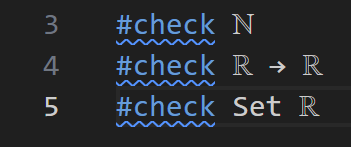
\includegraphics[width=0.5\linewidth]{basic_type_checks.png}
    \end{figure}
        
\end{frame}

\begin{frame}{Lean Syntax}

\begin{figure}
    \centering
    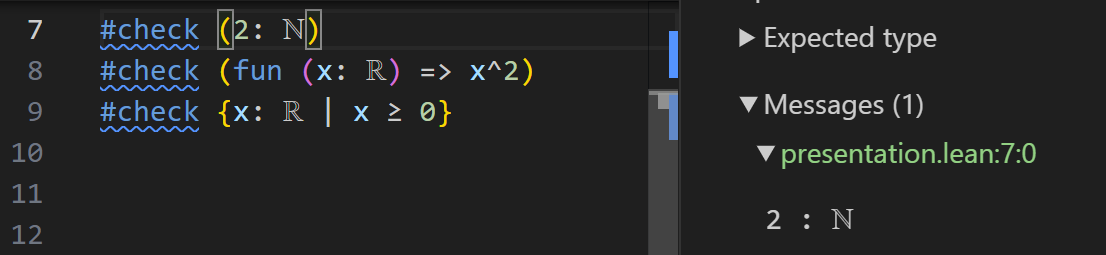
\includegraphics[width=1\linewidth]{name1.png}
\end{figure}

\end{frame}

\begin{frame}{Lean Syntax}

\begin{figure}
    \centering
    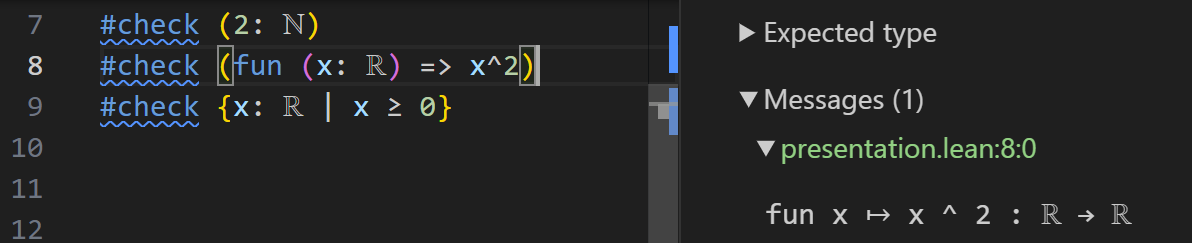
\includegraphics[width=1\linewidth]{name2.png}
\end{figure}

\end{frame}

\begin{frame}{Lean Syntax}

\begin{figure}
    \centering
    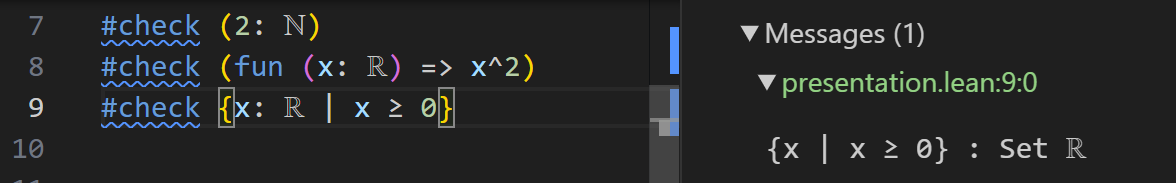
\includegraphics[width=1\linewidth]{name3.png}
\end{figure}

\end{frame}




%Sahan
\subsection{Propositions}

\begin{frame}{Propositions}


\begin{enumerate}
    \item A \textbf{proposition} is a mathematical statement converted to computer code
    \item \textbf{Prop} is a type
    \item Each proposition is an expression of type \textbf{Prop}
    \item Examples of propositions:
    \begin{itemize}
        \item $2 +2=4$
        \item $a < b$
        \item $\forall x, \exists \, y $ such that $2x = y$
    \end{itemize}



\end{enumerate}

\end{frame}



% \begin{frame}{Proofs}

% % slide is intentionally left mostly empty
% Expressions of type \textit{P} where \textit{P} is of type \textit{Prop} are proofs of \textit{P}. 
    




% \end{frame}

% \begin{frame}{Proofs}


% Expressions of type \textit{P} where \textit{P} is of type \textit{Prop} are proofs of \textit{P}. 
    
% \begin{enumerate}
%     \item Expressions of type $1<2$ prove that $1<2$.
%     \item Expressions of type $x+y=y+x$ prove that $x+y=y+x$. 
% \end{enumerate}


% \end{frame}

\begin{frame}{Proofs}


Expressions of type \textit{P} where \textit{P} is of type \textit{Prop} are proofs of \textit{P}. 
    
\begin{enumerate}
    \item Expressions of type $1<2$ prove that $1<2$.
    \item Expressions of type $x+y=y+x$ prove that $x+y=y+x$. 
\end{enumerate}


\begin{figure}
    \centering
    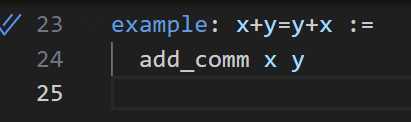
\includegraphics[width=1\linewidth]{example_proof_proofs_section.png}
\end{figure}

\end{frame}


% \subsection{Rewrite}
% \begin{frame}{Rewrite}

% \begin{figure}
% \centering
% 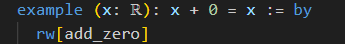
\includegraphics[scale=.78]{add_zero_example.png}


% \end{figure}

% \end{frame}

\section{Lean Examples}

\subsection{Basic Examples}

% katherine presents this slide 
\begin{frame}{Lean proof example: $x*x = x^2$}
\begin{figure}
    \centering
    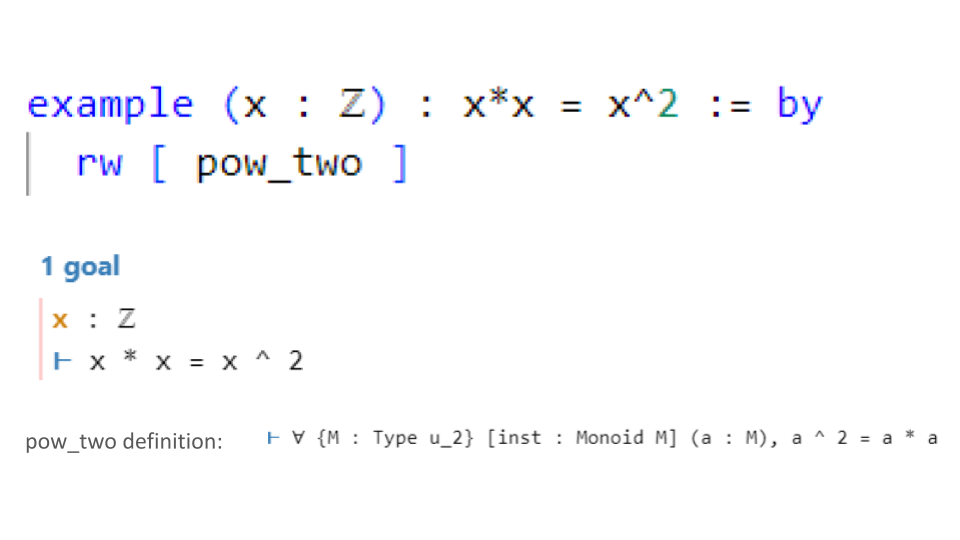
\includegraphics[scale=0.32]{xtimesxequalsx2.png}
\end{figure}
\end{frame}

%Clea
\begin{frame}{Lean proof example: $z*x*y*w=z*y*x*w$}

\begin{figure}
    \centering
    \includegraphics[width=1\linewidth]{Screenshot 2025-06-11 at 3.42.01 PM.png}
\end{figure}

\end{frame}


\subsection{Odd/Even Functions Proof}

%Clea
\begin{frame}{"Human" Proof of odd function times an odd function equals an even function}
\begin{enumerate}
\item Let $f(x)$ and $g(x)$ be odd functions, so that $f(x) = -f(-x)$ and $g(x) = -g(-x)$. Let $h(x) = f(x)*g(x)$. 
\item We want to show that $h(x)$ is even, or in other words, $h(x) = h(-x)$.
\item We have $h(x) = f(x) * g(x)$.
\item Using the definition of an odd function, $h(x) = -f(-x) * -g(-x)=f(-x)*g(-x)$.
\item We know $h(-x)= f(-x)*g(-x)$, so $h(x)=h(-x)$.
\item Thus, $h(x)$ is an even function.
\end{enumerate}
\end{frame}

%katherine presents this slide 
\begin{frame}{Our definition of even and odd functions}
\begin{figure}
    \centering
    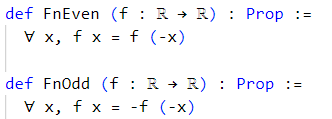
\includegraphics[scale=1]{ev_odd_def.png}
\end{figure}
\end{frame}

%Clea
\begin{frame}{Lean proof of odd function times an odd function equals an even function}

\begin{figure}
    \centering
    \includegraphics[width=1\linewidth]{Screenshot 2025-06-11 at 3.28.03 PM.png}
\end{figure}

\end{frame}

%katherine presents this slide 
\begin{frame}{Alternative lean proof of odd function times an odd function equals an even function}

\begin{figure}
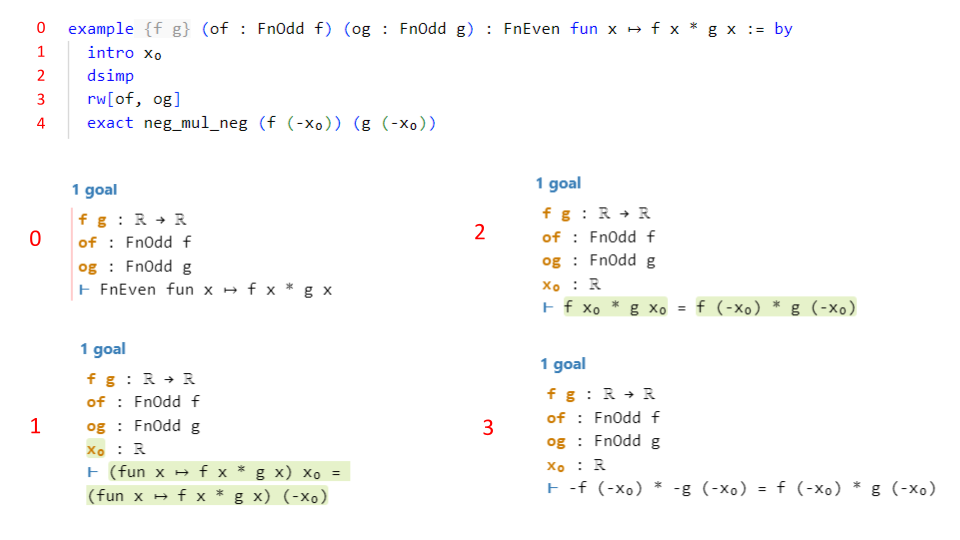
\includegraphics[scale=.32]{alt_ooe_pf.png}
\end{figure}
\end{frame}

\section{Future of Our Project}

%katherine presents this slide 
\begin{frame}{Potential applications}
\begin{enumerate}
\item Forms over finite fields
\item Quaternion algebra
\item Graph theory
\item The Grassmannian
\end{enumerate}
\end{frame}

%Clea
\begin{frame}{What's the point?}

\begin{enumerate}
   \item The transformation from "human mathematics" to "formalized mathematics" removes inferences from proofs, continuously checking that proofs are correct
   \item \textbf{mathlib} facilitates collaboration between mathematicians and allows proofs to be viewed by hundreds of scholars and students
   \item Proofs can be continuously modified and maintained by other mathematicians rather than becoming incompatible with other developments in Lean
   \item New methods to formalize a proof may have important pedagogical benefits
\end{enumerate}
\end{frame}

\section{Conclusion}

\begin{frame}{References}
\begin{enumerate}
\item Browning, T., \& Lutz, P. (2022). Formalizing Galois Theory. Experimental Mathematics, 31(2), 413-424.
\item Avigad, J. Buzzard, K. Lewis R. Y. Massot, P. (2020). \textit{Mathematics in Lean}. 
% I am not sure who the publisher for this book is. we should ask george if he knows. also this is me citing it as a book which i am not so sure if it is anymore 
\end{enumerate}
\end{frame}

\begin{frame}
	    \begin{center}
	        \textbf{Thank you!}\\
	        
	        Special thanks to Dr. George McNinch and the REU
         \bigbreak
         \LARGE
       
	    \end{center}
	\end{frame}
\end{document}